\documentclass{ltjsarticle}

\usepackage{tikz}
\usetikzlibrary{positioning,arrows.meta,shapes.geometric,backgrounds}

\begin{document}

Game 1 のゲーム木
\\\\

あいうえお。\\
かきくけこ。

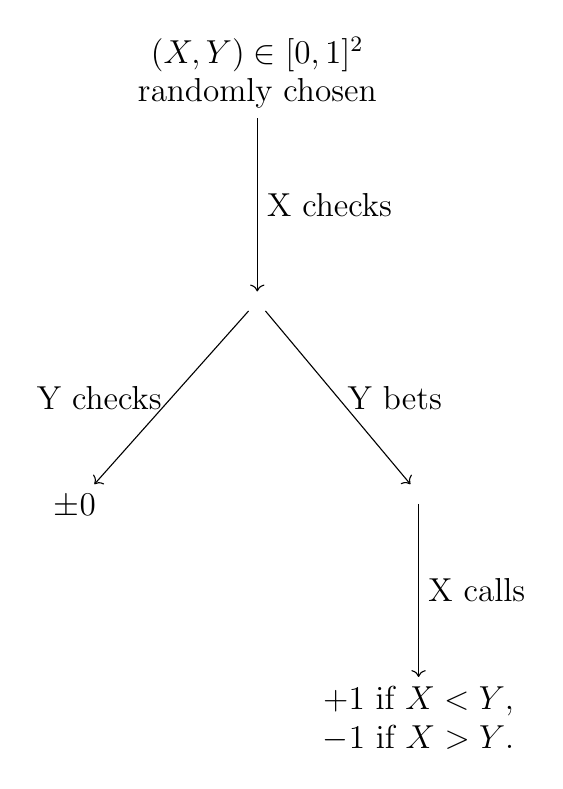
\begin{tikzpicture}

% nodes (manual positions for clearer layout)
\node[align=center, font=\large] (root) {$(X,Y)\in[0,1]^2$ \\randomly chosen};
\node[below=22mm of root] (xcheck) {};
\node[below left=22mm and 18mm of xcheck, font=\large] (ycheck) {$\pm 0$};
\node[below right=22mm and 18mm of xcheck] (ybets) {};
\node[align=center, below=22mm of ybets, font=\large] (xcall) {
$+1$ if $X < Y$, \\
$-1$ if $X > Y$.
};

% edges with labels
\draw[->] (root) -- (xcheck) node[midway,right, font=\large] {X checks};
\draw[->] (xcheck) -- (ycheck) node[midway,left, font=\large] {Y checks};
\draw[->] (xcheck) -- (ybets) node[midway,right, font=\large] {Y bets};
\draw[->] (ybets) -- (xcall) node[midway,right, font=\large] {X calls};

\end{tikzpicture}

\,\\\\
Strategy Structure
\\\\

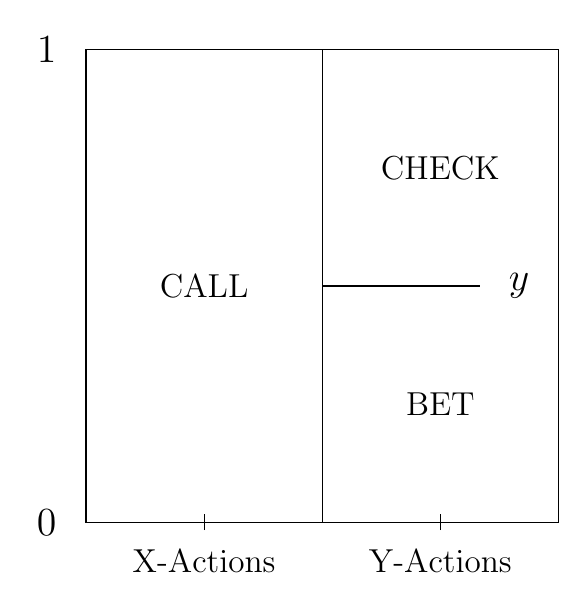
\begin{tikzpicture}

\draw (0,0) rectangle(6,6);
\draw (3,0) --(3,6);
\draw (3,3) --(5,3);

\draw (1.5,-0.1) --(1.5,0.1);
\draw (4.5,-0.1) --(4.5,0.1);

\node[font=\Large] at (-0.5,0) {$0$};
\node[font=\Large] at (-0.5,6) {$1$};
\node[font=\large] at (1.5, -0.5) {X-Actions};
\node[font=\large] at (4.5, -0.5) {Y-Actions};
\node[font=\Large] at (5.5, 3) {$y$};

\node[font=\large] at (1.5, 3) {CALL};
\node[font=\large] at (4.5, 4.5) {CHECK};
\node[font=\large] at (4.5, 1.5) {BET};

\end{tikzpicture}

\,\\\\
Strategy Graph
\\\\

\begin{tikzpicture}

\draw[->] (0,0) --(0,7);
\draw[->] (0,0) --(7,0);
\draw (0,6) --(6,6) --(6,0);
\draw (0,3) --(6,3);
\draw (0,0) --(3,3);
\draw[dashed] (3,3) --(6,6);
\draw[dashed] (3,0) --(3,3);

\node[font=\Large] at (7,-0.5) {X};
\node[font=\Large] at (-0.5,7) {Y};

\node[font=\Large] at (0,-0.5) {$0$};
\node[font=\Large] at (6,-0.5) {$1$};
\node[font=\Large] at (-0.5,0) {$0$};
\node[font=\Large] at (-0.5,6) {$1$};

\node[font=\Large] at (3,-0.5) {$y$};
\node[font=\Large] at (-0.5,3) {$y$};

\node[font=\Large] at (3,4.5) {$\pm 0$};
\node[font=\Large] at (3.7,1.3) {$-1$};
\node[font=\Large] at (1,2) {$+1$};

\end{tikzpicture}

\end{document}
